\chapter{Dataset}
- [-] explain where the dataset came from\\
- [-] chart of the timestamps distribuition\\
- [-] map of the class distribuition\\
- [-] map of train/validation/test dataset\\
- [x] table of distribuition (class + train/validation/test)\\

\section{Study Area}
The study area is centered on the city of Balaruc-les-Bains in south-eastern France. It borders the Mediterranean Sea and it has a surface of 100 $ km^2 $. It is a small but dense urban area surrounded by agricultural crops - mostly vineyards - and natural vegetation. Figure~ presents the GT map superposed on the Sentinel-2 image of the 23th January 2018. 

\begin{figure}[H]
  \centering
  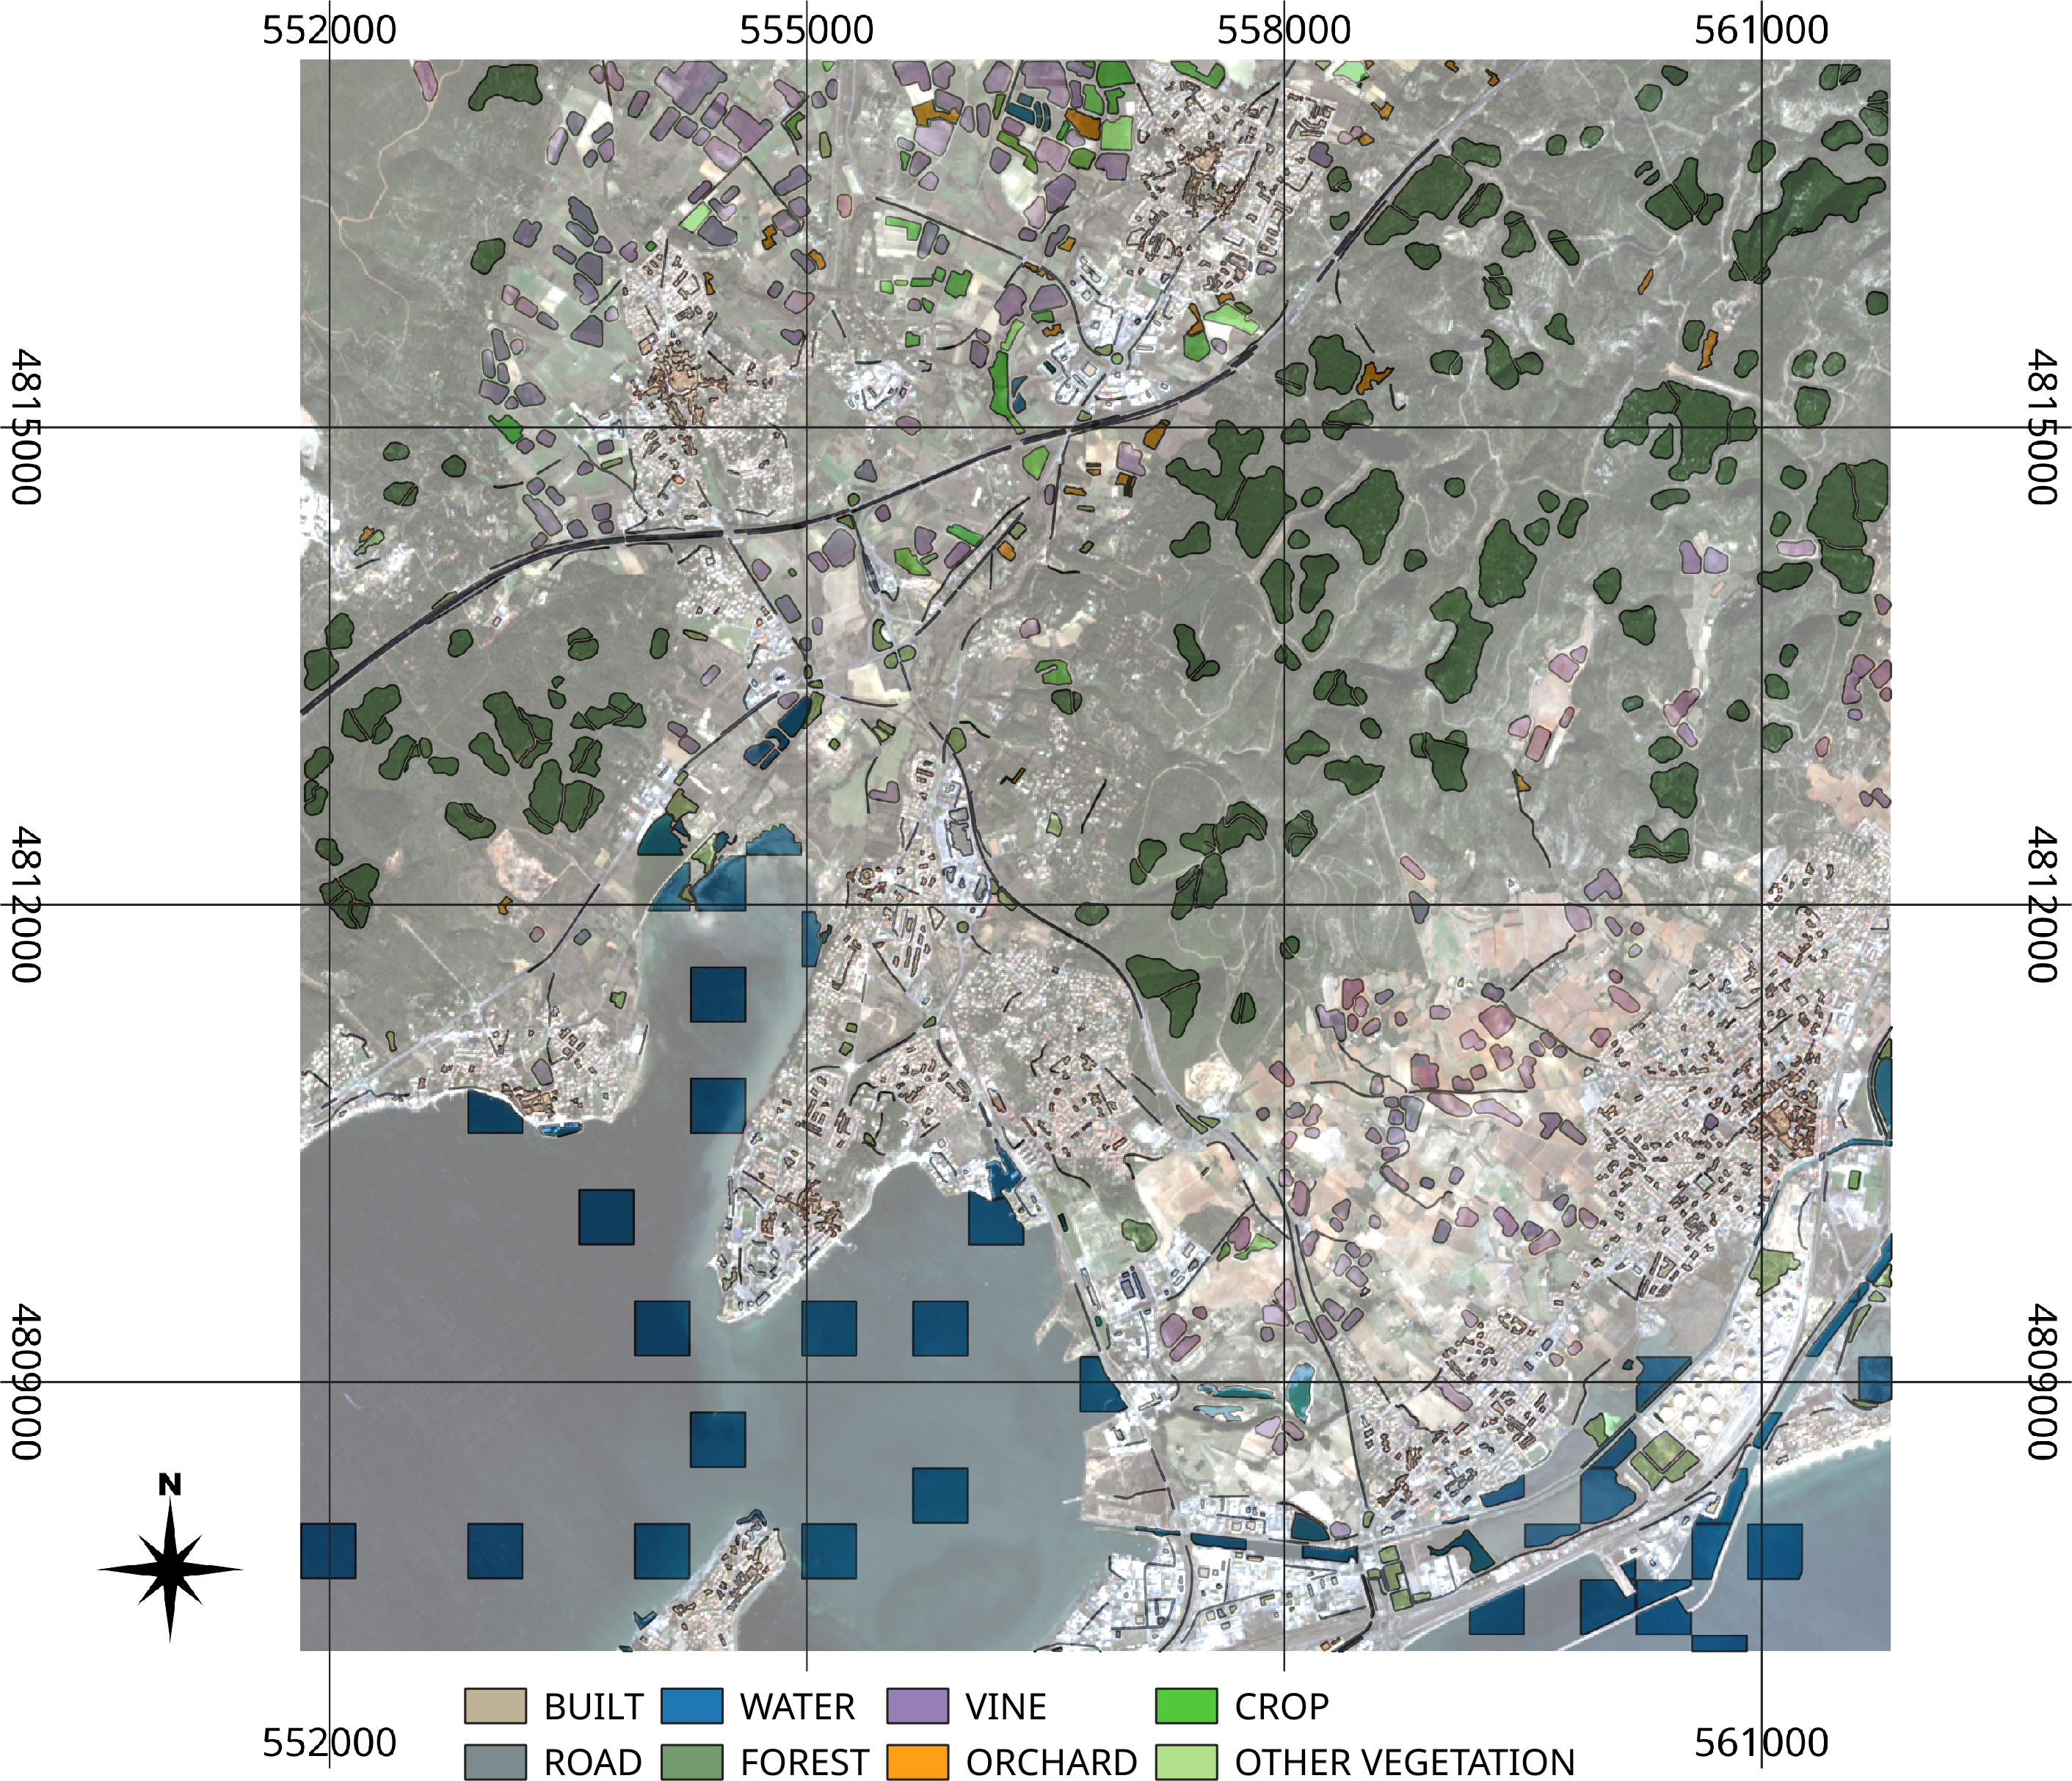
\includegraphics[width=1\textwidth]{BLC_20180123_SAT-GT_300dpi.png}
  \caption{Ground truth data superposed to a Sentinel-2 image.}
\end{figure}
% \begin{figure}[htb]
% \begin{minipage}[b]{1.0\linewidth}
%   \centering
%     \centerline{\epsfig{figure="Figures/BLC_20180123_SAT-GT_300dpi.png",width=8cm}}
% \end{minipage}
% \caption{Ground truth data superposed to a Sentinel-2 image.}
% \label{fig:gtmap}
% \end{figure}


\textit{Satellite Image Time Series:} We collect satellite image time series of Sentinel-2 imagery spanning the years 2018 and 2019. For each year, we retain 24 images to guarantee a similar temporal sampling step. Images were also chosen with the aim to be representative of the temporal (annual) evolution of the land covers associated to the study area as well as to filter out images that were seriously impacted by cloud phenomena. Figure~ depicts the acquisition dates of the two Sentinel-2 satellite image time series. 

\begin{figure}[H]
  \centering
  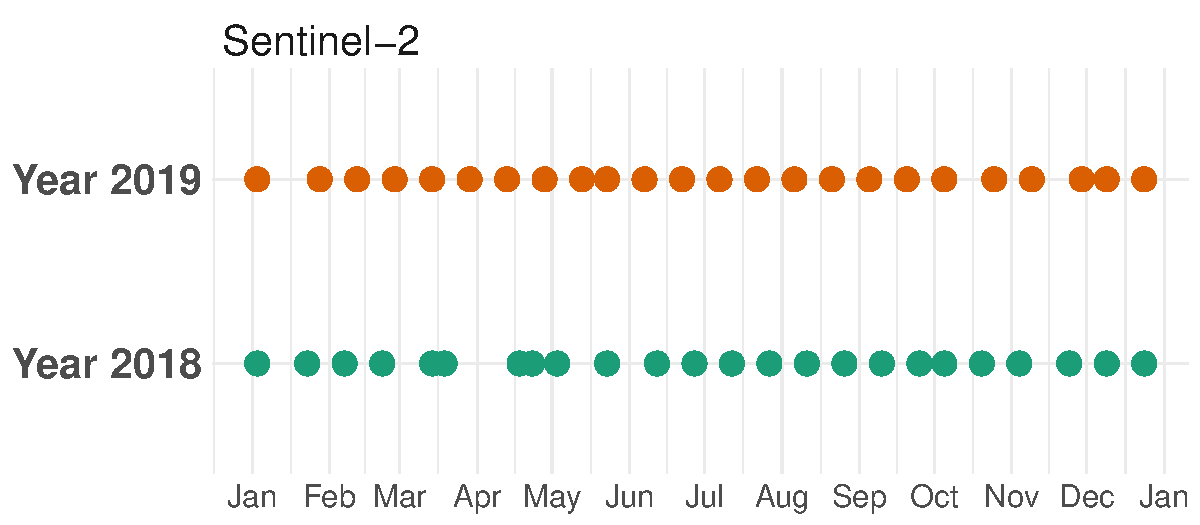
\includegraphics[width=1\textwidth]{2018-2019_chronologie_EN.pdf}
  \caption{Acquisition dates of each Satellite Image Time Series.}
\end{figure}
% \begin{figure}[htb]
% \begin{minipage}[b]{1.0\linewidth}
%   \centering
%     \centerline{\epsfig{figure="Figures/2018-2019_chronologie_EN.pdf",width=8.5cm}}
% \end{minipage}
% \caption{Acquisition dates of each Satellite Image Time Series.}
% \label{fig:chronology}
% \end{figure}

All images were provided by the THEIA pole platform~ at level-2A in top of canopy reflectance values with associated cloud masks. Only 10-m spatial resolution bands (Blue, Green, Red and Near infrared spectrum) were considered in this analysis. A preprocessing was performed over each band to replace cloudy pixel values as detected by the available cloud masks through a linear multi-temporal interpolation (cf. temporal gap-filling~. The entire study site is enclosed in the Sentinel-2 tile 31TEJ with relative orbit n°8.

\textit{Ground truth data:} The GT data for 2018 was built from various sources: the \textit{Registre Parcellaire Graphique} (RPG) reference data (the French land parcel identification system), the French National Geographic Institute \textit{‘BD-Topo \& BD Forêt’} and the visual interpretation of a SPOT 6 image (to assess and enrich the GT data) as well. The GT was assembled in Geographic Information System (GIS) vector file, containing a collection of polygons, each attributed with a land cover category. Statistics about the GT data are reported in Table~\ref{tab:gt}.
It was assumed that this GT data is also valid for 2019 because no significant change has occurred in this area between 2018 and 2019. 

\begin{table}[htb]
\centering
\scriptsize
\begin{tabular}{ |l|c|r|r| }
 \hline
 Class Name & Class ID. & \# Polygons & \# Pixels \\ 
 \hline
 BUILT & 1 & 712 & 10411\\
 ROAD & 2 & 328 & 5165 \\
 WATER & 3 & 82 & 32095 \\  
 FOREST & 4 & 172 & 49175 \\  
 VINE & 5 & 223 & 28630 \\
 ORCHARD & 6 & 32 & 2075 \\
 CROP & 7 & 39 & 5205 \\
 OTHER VEGETATION & 8 & 56 & 4812 \\
 \hline
 & Total & 1644 & 137568 \\
 \hline
\end{tabular}
\caption{Ground truth statistics.}
\label{tab:gt}
\end{table}

\begin{table}[]
  \centering
  \begin{tabular}{lllllll}
  \hline
  Class   & \multicolumn{2}{l}{Train} & \multicolumn{2}{l}{Validation} & \multicolumn{2}{l}{Test} \\ \cline{2-7} 
          & Pixels  & (\%) & Pixels    & (\%)    & Pixels & (\%) \\ \hline
  Built   & 6,381   & 8.1             & 1,775     & 6.1                & 2,256  & 7.7             \\
  Road    & 3,014   & 3.8             & 1,323     & 4.5                & 828    & 2.8             \\
  Water   & 16,534  & 20.9            & 6,856     & 23.4               & 8,705  & 29.8            \\
  Forest  & 29,654  & 37.4            & 10,739    & 36.7               & 8,782  & 30.1            \\
  Vine    & 16,399  & 20.7            & 6,002     & 20.5               & 6,266  & 21.5            \\
  Orchard & 1,464   & 1.8             & 218       & 0.7                & 393    & 1.3             \\
  Crop    & 2,598   & 3.3             & 1,370     & 4.7                & 1,237  & 4.2             \\
  Other   & 3,147   & 4.0             & 966       & 3.3                & 699    & 2.4             \\ \hline
  Total   & 79,191  & 100             & 29,249    & 100                & 29,166 & 100            
  \end{tabular}
  \caption{Number of polygons and pixels for each class.}
\end{table}

